\documentclass[10pt,twocolumn]{article}
\usepackage[margin=0.75in]{geometry}
\usepackage{graphicx,booktabs,amsmath,url,xcolor}
\usepackage[hidelinks]{hyperref}
\title{Seed Sensitivity of Composite Video-Quality Metrics:\\
A Reproducibility Study of MiniMax-H3 under Sci-VBench VT}
\author{Anonymous}
\date{}

\begin{document}
\maketitle

\begin{abstract}
Composite video-quality metrics such as the VT score of Sci-VBench aggregate
six component metrics and are increasingly used to rank video-generation models.
We reproduce the released MiniMax-H3 VT scores to $\sim$10$^{-6}$ numerical
precision, then show that single-seed VT comparisons are dominated by seed
noise: across 16 prompts $\times$ 12 seeds, the within-prompt seed SD of VT is
$0.051$ for MiniMax-H3, so the paired SE of a single-seed two-model mean
difference ($\pm0.035$ at 95\%) is 5.3$\times$ the $0.0066$ median gap between
adjacent released models. The largest contributor is Dynamic Degree (DD),
whose binarised value flips in 27.5\% of the 1{,}056 seed pairs over 12 seeds
per prompt (Wilson 95\% CI $[24.9\%, 30.2\%]$). Cross-model replications with Wan2.1-Fun and LTX-Video-2B (each 192 videos
over 12 seeds) find DD flip rates of 17.2\% (CI $[15.1\%, 19.6\%]$) and 11.9\%
(CI $[10.1\%, 14.0\%]$) --- model-specific but always substantial --- with
prompt/seed variance nearly equal in all three (ANOVA ICC$_{\text{prompt}}$
0.46--0.56), consistent with seed sensitivity being a property of the metric
pipeline rather than of one model. A descriptive join with 2{,}392 human expert scores shows pooled rank
correlation $-0.04$ between VT and the expert LPF dimension
(cluster-bootstrap CI $[-0.09, +0.01]$). We recommend multi-seed reporting
with per-prompt dispersion and care when interpreting thresholded motion
metrics.
\end{abstract}

\section{Introduction}
Leaderboards for text-to-video models increasingly rely on composite
auto-evaluation scores. Sci-VBench VT averages six VBench-style components
(subject/background consistency, motion smoothness, dynamic degree, aesthetic
and imaging quality). Model rankings are published to third-decimal precision,
typically from a single generation seed per prompt. Following the precedent of
\emph{Deep RL that matters}~\cite{henderson2018}, we ask how much of a
single-seed VT score is signal.

\textbf{Contributions.}
(1)~A numerical reproduction ($\sim$10$^{-6}$) of the released 150-video MiniMax-H3 VT results
(Sec.~\ref{sec:e2}).
(2)~A seed-power study: 16 prompts $\times$ 12 seeds on H3
(Sec.~\ref{sec:e3}).
(3)~Cross-model replications on Wan2.1-Fun and LTX-Video-2B under their official protocols
(Sec.~\ref{sec:e4}).
(4)~A descriptive human-score join (Sec.~\ref{sec:human}).

\section{Related Work}
Video-generation evaluation suites include
VBench~\cite{vbench}, VBench++~\cite{vbenchpp}, VBench-2.0~\cite{vbench2},
EvalCrafter~\cite{evalcrafter} and VideoPhy~\cite{videophy}; Sci-VBench~\cite{scivbench}
targets knowledge- and reasoning-intensive scientific prompts. Motion-sensitive
components inherit a long line of spatio-temporal quality
assessment~\cite{motiontuned}. Reproducibility of stochastic training/evaluation
pipelines is well studied in RL~\cite{henderson2018} and in ML benchmarks
generally~\cite{bouthillier2021variance,keeling2024quantifying}, and
NLG-specific reproducibility efforts (ReproGen, QRA++,
quantified-reproducibility protocols)~\cite{reprogen2021,qra2025} document
similar variance-driven instability in text metrics. Metric-reliability studies
for text-to-video are emerging~\cite{t2vmetricreliability}; our contribution is
a seed-resolved, per-metric decomposition on a released, fully reproducible
leaderboard. Human-preference data for video generation is studied
in~\cite{videofeedback}. To our knowledge the
seed-sensitivity of \emph{composite} scores relative to \emph{model gaps} has
not been quantified for these suites.

\section{Setup}
\textbf{Evaluator.} Sci-VBench VT runner at pinned commit
\texttt{e8cb3988}: six metrics (subject/background consistency, motion
smoothness, dynamic degree DD, aesthetic quality, imaging quality), unweighted
mean $=$ VT. Human-score analyses use the released expert dimensions (LPF =
Low-level Perceptual Fidelity, one of four expert dimensions, each 1--5). ICC$_{\text{prompt}}$ denotes a
balanced one-way ANOVA variance-component intraclass correlation over prompts.
Hardware: one H100; evaluator versions pinned in the released scripts.
\textbf{H3.} Official \texttt{MiniMax-H3} weights (1344$\times$768, 24\,FPS,
5.175\,s). \textbf{Wan.} Wan2.1-Fun-V1.1-1.3B-InP via the official
VideoX-Fun \texttt{predict\_t2v} entry (832$\times$480, 16\,FPS, 81 frames
$\approx$ 5.06\,s, 50 steps, TeaCache at recommended settings); protocol
differences are explicit and we never compare absolute scores across models.
All generation/evaluation scripts, per-video JSONs and audit notes are
released.

\section{E2: Reproducing released scores}\label{sec:e2}
We re-evaluated the 150 released H3 test-mini videos with the pinned evaluator.
\begin{table}[t]
\centering\small
\begin{tabular}{lcc}
\toprule
Metric & median $|\Delta|$ & exact match\\
\midrule
SC & $1.45\mathrm{e}{-8}$ & --\\
BC & $2.44\mathrm{e}{-5}$ & --\\
MS & $1.82\mathrm{e}{-6}$ & --\\
DD & $0$ & 149/150\\
AQ & $6.17\mathrm{e}{-6}$ & --\\
IQ & $1.64\mathrm{e}{-5}$ & --\\
VT & $6.15\mathrm{e}{-6}$ & --\\
\bottomrule
\end{tabular}
\caption{Reproduction accuracy: released vs.\ re-evaluated scores over the
150 H3 test-mini videos. Re-run aggregate VT $0.735706$ vs.\ released $0.734596$.}
\label{tab:e2}
\end{table}
Median absolute deltas in Table~\ref{tab:e2}; the reproduction gate passed and
all later experiments use this stack. The re-run aggregate VT is $0.735706$
vs.\ released $0.734596$: the $0.0011$ difference is exactly the single
mismatched DD cell (a DD flip changes that video's VT by $1/6$), and all
continuous metrics agree at the $10^{-6}$ level.

\section{E3: Seed power on H3}\label{sec:e3}
16 prompts $\times$ 12 seeds (192 videos, verbatim Sci-VBench prompts):
\begin{itemize}\itemsep2pt
\item DD pairwise flip $290/1056 = 27.46\%$ (Wilson 95\% CI $[24.9\%, 30.2\%]$); 12/16 prompts flip at least once.
\item Within-prompt VT SD: mean $0.0509$ (population SD over 12 seeds, matching Table~\ref{tab:icc}), max $0.0841$; DD SD $0.3012$.
\item The released leaderboard (eight models with full 1{,}253-video coverage,
including H3 at rank 4) has median adjacent-model VT gap $0.0066$
(max $0.0183$); the paired SE of a single-seed two-model mean difference is
$\pm0.035$, 5.3$\times$ that median gap.
\item $k$-seed averaging: SE $0.0211 \rightarrow 0.0164$ for $k{=}1..12$;
averaging does not remove the noise floor.
\item \emph{Threshold invariance}: within-prompt DD distributions are nearly
bimodal (saturated at 0 or 1), and the flip rate is unchanged for any
binarization threshold in $[0.05, 0.60]$ --- the phenomenon is not an artifact
of threshold choice.
\item \emph{Rank instability}: for each of the 66 seed pairs, ranking the 16
prompts by single-seed VT yields mean Spearman $\rho=0.54$ between the two
rankings (min $-0.06$) and a mean absolute rank displacement of $3.2/16$
positions --- seed choice alone reshuffles prompt-level rankings.
\end{itemize}
\begin{figure}[t]
\centering
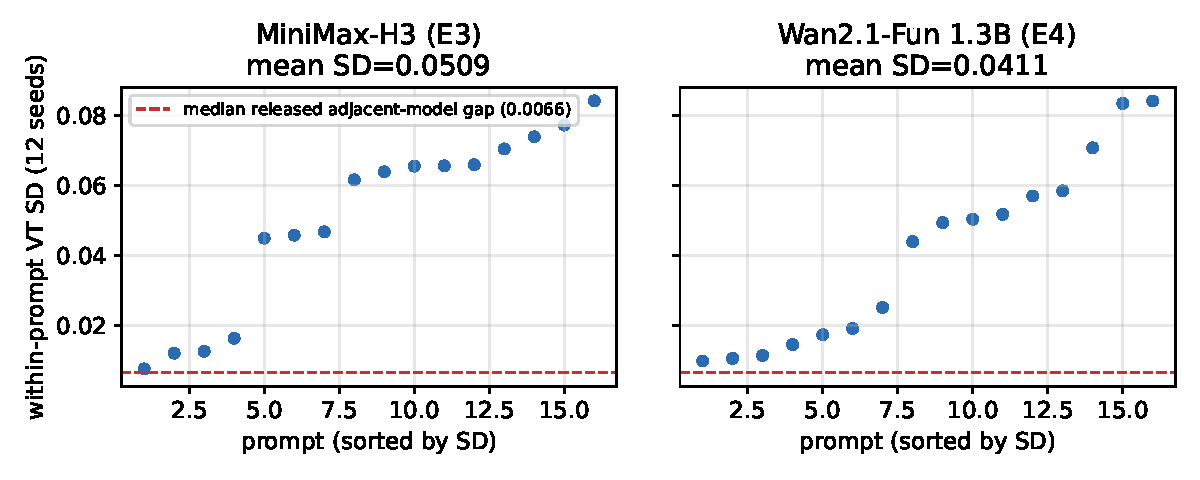
\includegraphics[width=\linewidth]{fig1_within_prompt_sd.pdf}
\caption{Within-prompt VT SD over 12 seeds (16 prompts), H3 (left) and
Wan2.1-Fun (right); dashed line: median released adjacent-model gap ($0.0066$).}
\label{fig:sd}
\end{figure}
\begin{figure}[t]
\centering
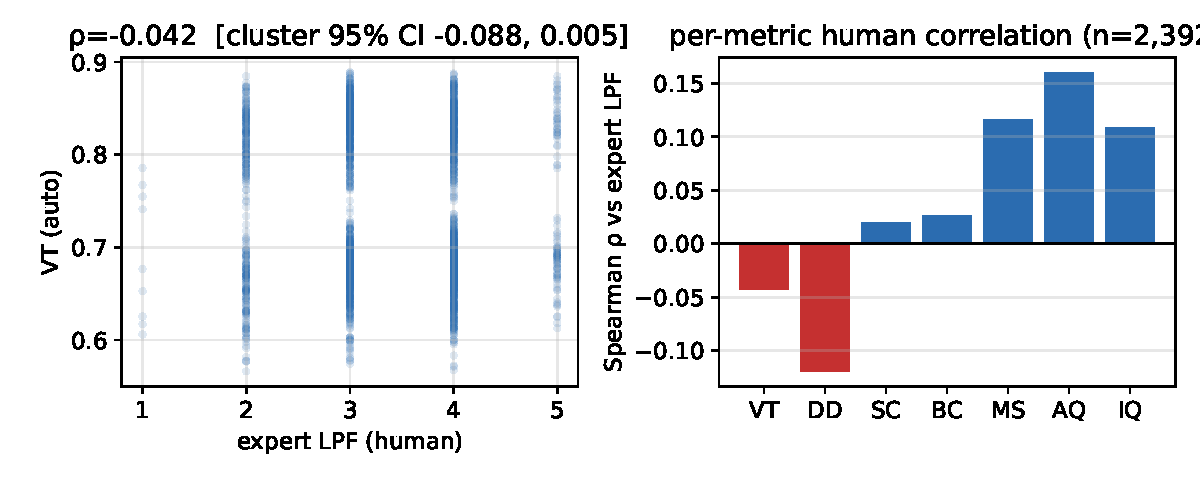
\includegraphics[width=\linewidth]{fig3_human_join.pdf}
\caption{Human-score join: VT vs.\ expert LPF scatter (left) and per-metric
Spearman $\rho$ (right). DD correlates negatively with expert scores.}
\label{fig:human}
\end{figure}
\begin{figure}[t]
\centering
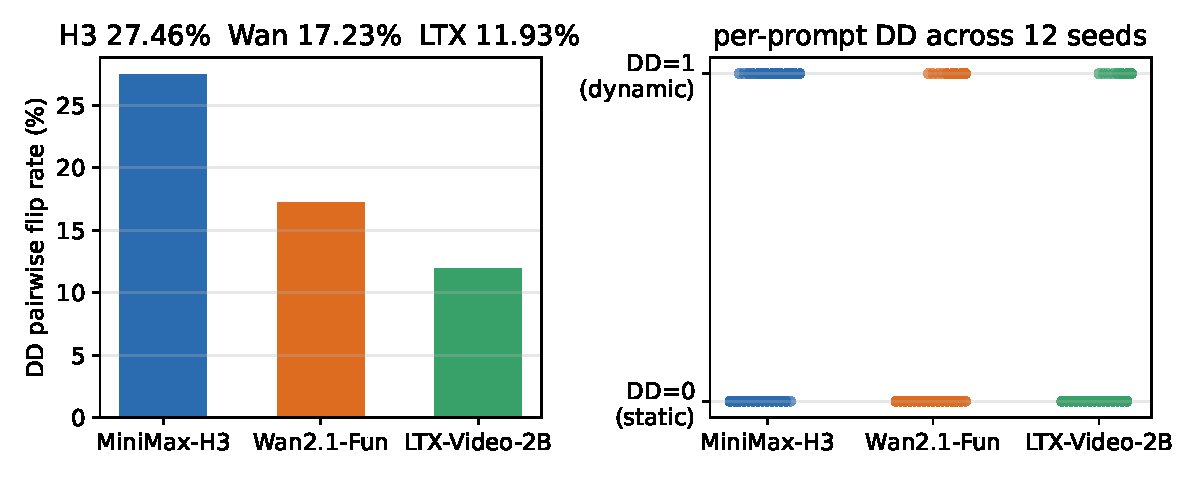
\includegraphics[width=\linewidth]{fig2_dd_flip.pdf}
\caption{DD seed instability: flip rates and per-prompt DD across seeds.}
\label{fig:dd}
\end{figure}

\section{E4: Cross-model replication}\label{sec:e4}
Wan2.1-Fun 1.3B, 16$\times$12 under its official protocol (192 unique videos,
0 failures; DD mean $0.188$): flip rate $182/1056=17.23\%$ (CI $[15.1\%, 19.6\%]$; disjoint from H3's), any-flip $9/16$,
within-prompt VT SD $0.0411$ (max $0.0841$). The rank-instability statistic
replicates: mean between-seed ranking $\rho=0.54$ (min $0.06$), mean rank
displacement $3.3/16$ over the 66 pairs. Variance decomposition
(Table~\ref{tab:icc}): H3 ICC$_{\text{prompt}}{=}0.56$; Wan $0.48$, i.e.\
prompt and seed contributions overlap within bootstrap uncertainty. Within-prompt SD is almost
similar across the three models ($0.051$ / $0.041$ / $0.040$; population-SD means) despite very different
architectures, samplers and resolutions --- evidence that the noise floor is a
property of the metric pipeline, with the binarised DD as the dominant carrier
on H3 (Fig.~\ref{fig:dd}).

Table~\ref{tab:e5} summarises the three models. \paragraph{E5: third model.}
We repeat the full protocol on LTX-Video-2B (same 16 prompts, 12 seeds,
832$\times$480, 81 frames @16\,fps, 40 steps): 192/192 videos, 0 failures.
DD flip $126/1056 = 11.93\%$ (CI $[10.1\%, 14.0\%]$; disjoint from H3's);
any-flip $7/16$; within-prompt VT SD $0.040$ (max $0.075$);
ICC$_{\text{prompt}} = 0.46$ $[0.10, 0.71]$; mean between-seed ranking
$\rho = 0.46$ (min $-0.10$), displacement $3.5/16$. All three models therefore
exhibit the same qualitative phenomena: a $\sim$0.04--0.05 within-prompt VT
noise floor, a binary DD flag that flips across seeds at a model-specific but
always substantial rate, and near-equal prompt/seed variance shares. The
subset-SE validation also extends: LTX's empirical SEs exceed the i.i.d.\
prediction by $1.3$--$1.7\times$ at $s{\in}\{2,3,4,6\}$ (vs.\ $0.7$--$0.9\times$
for H3 and $0.9$--$1.2\times$ for Wan), so the i.i.d.\ noise model is
model-dependent in detail --- and where it errs on LTX, it is
\emph{optimistic}, strengthening the resolution conclusions.

\begin{table}[t]
\centering\small
\begin{tabular}{lccccc}
\toprule
 & DD flip (95\% CI) & any-flip & VT SD & ICC$_{\text{prompt}}$ & rank $\rho$\\
\midrule
MiniMax-H3   & 27.5\% [24.9, 30.2] & 12/16 & 0.051 & 0.56 [0.30, 0.72] & 0.54\\
Wan2.1-Fun   & 17.2\% [15.1, 19.6] & 9/16 & 0.041 & 0.48 [0.22, 0.65] & 0.54\\
LTX-Video-2B & 11.9\% [10.1, 14.0] & 7/16 & 0.040 & 0.46 [0.10, 0.71] & 0.46\\
\bottomrule
\end{tabular}
\caption{Cross-model summary (all: 16 prompts $\times$ 12 seeds $=$ 1{,}056 seed
pairs; rank $\rho$ averaged over the 66 seed pairs).}
\label{tab:e5}
\end{table}
\begin{table}[t]
\centering\small
\begin{tabular}{lcccc}
\toprule
 & between-prompt SD & within-prompt SD & ICC$_{\text{prompt}}$ & 95\% CI\\
\midrule
H3           & 0.0636 & 0.0509 & 0.56 & [0.30, 0.72]\\
Wan2.1-Fun   & 0.0463 & 0.0411 & 0.48 & [0.22, 0.65]\\
LTX-Video-2B & 0.0414 & 0.0403 & 0.46 & [0.10, 0.71]\\
\bottomrule
\end{tabular}
\caption{VT variance decomposition (16 prompts $\times$ 12 seeds, same evaluator). ICC from balanced one-way ANOVA variance components; CI from bootstrap over the 16 prompts (2{,}000 resamples). H3's larger between-prompt SD reflects domain-skewed pilot prompts.}
\label{tab:icc}
\end{table}

\section{Human scores (descriptive)}\label{sec:human}
Joining all 2{,}392 human expert scores (the released expert dimensions,
including LPF) with VT results: pooled
Spearman$(\text{VT}, \text{LPF}) = -0.0423$; a cluster bootstrap over the 150
prompt topics ($B{=}2000$) gives 95\% CI $[-0.088, +0.005]$, i.e.\
indistinguishable from zero. DD shows a negative rank association with LPF
($-0.119$). We report these as descriptive associations (Fig.~\ref{fig:human}); no claim
about the construct validity of individual metrics is made.

\section{Discussion}
Adjacent-model gaps sit far below the noise floor of single-seed
comparisons: the median gap ($0.0066$) is 5.3$\times$ smaller than the $\pm0.035$
single-seed paired 95\% half-width.
\emph{Resolution analysis:} in a paired comparison over the same $P{=}16$
prompts, the prompt effect cancels and the paired-difference SE is
$\sigma_{sp}\sqrt{2/(Ps)}$ with $\sigma_{sp}$ the within-prompt seed SD
($0.051$ H3, $0.041$ Wan). Even with 6 seeds (half the budget) the 95\% half-width
($\pm0.015$ H3, $\pm0.011$ Wan) still exceeds the median adjacent gap;
resolving it at 95\% requires ${\sim}30$ seeds per prompt on H3
(${\sim}17$ on Wan), and resolving the minimum gap ($0.003$) requires
${\sim}154$ and ${\sim}84$ respectively --- or proportionally more prompts.
The i.i.d.-noise model is empirically checked: with 12 seeds, subset-based
empirical SEs at $s{\in}\{2,3,4,6\}$ fall within $0.66\times$--$1.23\times$ the
prediction for H3 and Wan, and $1.31\times$--$1.70\times$ for LTX --- the only
model where the model errs, and it errs \emph{optimistic}, so the resolution
conclusions are conservative in every case.
We recommend: (i)~report
multi-seed mean and per-prompt dispersion; (ii)~present DD separately from the
continuous composite, or replace its thresholding; (iii)~treat
sub-0.01 VT improvements as noise until multi-seed CIs are shown.

\section{Limitations}
One evaluator stack; 16$\times$12 scale on three open models spanning two families (2B-scale
Wan/LTX vs.\ H3); proprietary frontier generators are untested; Wan replication aligns duration and prompts but not
resolution/sampler, and runs under TeaCache caching, so it is a
metric-behaviour replication, not a same-config quality comparison; the
resolution analysis assumes homoscedastic, seed-independent noise (within-prompt SD is in fact heteroscedastic: max $0.084$ vs.\ mean $0.051$); the
human-score join is pooled and descriptive.

\bibliographystyle{plain}
\begin{thebibliography}{9}
\bibitem{bouthillier2021variance}
S.~Bouthillier et al., ``Accounting for variance in machine learning benchmarks,''
in \emph{Proc.\ MLSys}, 2021.

\bibitem{keeling2024quantifying}
J.~Keeling et al., ``Quantifying variance in evaluation benchmarks,'' \emph{arXiv:2406.10229}, 2024.

\bibitem{reprogen2021}
S.~Baluja et al., ``The ReproGen shared task on reproducibility of human evaluations in NLG,'' in \emph{Proc.\ INLG}, 2021.

\bibitem{qra2025}
``QRA++: Quantified reproducibility assessment for common types of results in natural language generation,'' \emph{arXiv:2505.01704}, 2025.

\bibitem{t2vmetricreliability}
``Evaluating the evaluators: Metric reliability and agreement in text-to-video generation,'' 2026.

\bibitem{henderson2018} P. Henderson et al. Deep reinforcement learning that matters. AAAI 2018.
\bibitem{vbench} Z. Huang et al. VBench: Comprehensive benchmark suite for video generative models. CVPR 2024.
\bibitem{vbenchpp} Z. Huang et al. VBench++: Comprehensive and versatile benchmark suite. TPAMI 2025.
\bibitem{vbench2} Z. Huang et al. VBench-2.0: Advancing video generation benchmark suite for intrinsic faithfulness. arXiv:2503.21755, 2025.
\bibitem{evalcrafter} Z. Liu et al. EvalCrafter: Benchmarking and evaluating large video generation models. CVPR 2024.
\bibitem{videophy} H. Bansal et al. VideoPhy: Evaluating physical commonsense for video generation. ICLR 2025.
\bibitem{scivbench} Sci-VBench: Evaluating knowledge- and reasoning-intensive video generation in science domains. arXiv:2608.09873, 2026.
\bibitem{motiontuned} Motion tuned spatio-temporal quality assessment of natural videos. IEEE TIP 2009.
\bibitem{videofeedback} Improving video generation with human feedback. NeurIPS 2025.
\end{thebibliography}

\end{document}
